
\chapter{Design}

In this chapter is described design of solution and explained decisions that were made.
Implementation details are described in Chapter \ref{chap:implementation}.

In the first section is described design of \lsystem processing library.
Library process input with component-based approach.
Core of the library is responsible for creating system of connected components (components graph) but processing of \lsystem itself is fully under control of components.
Components can be created by user which bring freedom to \lsystem processing.

Library it will contain predefined components to be possible to process \lsystems without need of creating custom components.
Design of these components is described in the second section.
These components will also serve as an example for users who want to implement their own processing system.

In the third section is described design of online web user interface.
It uses library and components to process input so it will also serve as an example of usage.



\section{\lsystem processing library design}

\lsystem processing library design will provide application interface (API) for processing of \lsystems.
The main feature will be extensibility....






















\section{Processing system}
\label{sec:design-components}

As discussed in the previous chapter, the processing system of the library relies on the components.
The core of the library is responsible for just creating the component graph.
The processing of an \lsystem and production of results is fully under the control of the component graph.
This gives absolute freedom to the user in implementing the process system.

However it is hard to design and implement the whole \lsystem processing system from scratch.
The library contains a rich set of predefined components from which can be assembled many different component graphs.
The predefined components have a general interface which allows the user to reuse or extend them in order to add new functionality with a minimum of effort.


\subsection{Basic component system}

The component system designed in this section is primarily used for processing \lsystems to produce 2D and 3D graphics in the web interface.
However, the component system is designed to be extensible to any output type.

\lsystems are generally processed in two phases.
The first phase is rewriting where the axiom (the initial string of symbols) is rewritten by the rewrite rules, and the second phase is interpreting the resulting string of symbols.
This can be done with two components, the Rewriter -- which is responsible for rewriting the \lsystem to a given iteration -- and the Interpreter -- which is responsible for interpreting symbols and producing output (Fig. \ref{fig:simpleSystem}).

\begin{figure}[h!]
	\centering
	\begin{tikzpicture}[->,auto,node distance=3cm,>=latex,shorten >=2pt]
		\node (in) [coord] {};
		\node (rw) [block, right of=in] {Rewriter};
		\node (int) [block, right=1cm of rw] {Interpreter};
		\node (out) [coord, right of=int] {};
		
		\draw (in) -- node {input} (rw);
		\draw (rw) -- (int);
		\draw (int) -- node {output} (out);
	\end{tikzpicture}
	\caption{Simple \lsystem processing system}
	\label{fig:simpleSystem}
\end{figure}

However the components in the system in \autoref{fig:simpleSystem} have too many tasks to do, and thus they will be complicated to implement and hard to extend and test.

The system in \autoref{fig:advancedSystem} was created by a subdivision of the previous system.
The Rewriter component was split to the Rewriter and the Iterator.
The (new) Rewriter will just do the rewriting of some given symbols and the Iterator will control the iterating of the \lsystem (repetitive rewriting).
The Interpreter component was split to the Interpreter and the Renderer.
The (new) Interpreter will handle the interpreting of symbols: which means keep position of the virtual "turtle" in space, saving and loading of states, etc.
The Renderer will just produce the output.
If we need to create a different output type we only have to implement the new renderer component and the rest of the system will remain unchanged.

\begin{figure}[h!]
	\centering
	\begin{tikzpicture}[->,auto,node distance=3cm,>=latex,shorten >=2pt]
		\node (rw) [block] {Rewriter};
		\node (iter) [block, right of=rw] {Iterator};
		\node (in) [coord, above of=iter, node distance=15mm] {};
		\node (inter) [block, right of=iter] {Interpreter};
		\node (rend) [block, right of=inter] {Renderer};
		\node (out) [coord, right of=rend] {};
		
		\draw (rw) to[bend left=40] (iter);
		\draw (iter) to[bend left=40] (rw);
		\draw (in) -- node {input} (iter);
		\draw (iter) -- (inter);
		\draw (inter) -- (rend);
		\draw (rend) -- node {output} (out);
	\end{tikzpicture}
	\caption{Subdivided \lsystem processing system}
	\label{fig:advancedSystem}
\end{figure}


\subsection{Component system extensions}
\label{sec:caller}

The system in \autoref{fig:callerComponent} can be enhanced even more.
Every component that interprets \lsystem symbols needs to translate symbols to interpretation methods.
The translation can be implemented by every component individually.
However, the translation can be done by a specialized component called the \emph{Interpreter caller}.
This component can be smart enough to explore all the components in the system, find all the interpretation methods of all components and do translation automatically.
This causes an automatic "connection" of all interpreters to the interpreter caller.

More interpreters can be used to advantage: for example, for processing \lsystems which interact with themselves or their Environment \cite{MP96}.
One interpreter actually creates the result model and the second interpreter simulates the environment.

\begin{figure}[h!]
	\centering
	\begin{tikzpicture}[->,auto,node distance=3cm,>=latex,shorten >=2pt]
		\node (iter) [block] {Iterator};
		\node (in) [coord, above of=iter, node distance=15mm] {};
		\node (rw) [block, below of=iter, node distance=20mm] {Rewriter};
		\node (caller) [blockx, right of=iter, node distance=35mm] {Interpreter caller};
		\node (inter) [block, right of=caller, node distance=40mm] {Interpreter};
		\node (env) [block, below of=inter, node distance=20mm] {Environment module};
		\node (rend) [block, right of=inter] {Renderer};
		\node (out) [coord, right of=rend] {};
		
		\draw (rw) to[bend left=40] (iter);
		\draw (iter) to[bend left=40] (rw);
		\draw (in) -- node {input} (iter);
		\draw (iter) -- (caller);
		\draw [dashed] (caller) -- (inter);
		\draw [dashed] (caller) -- (env);
		\draw (inter) -- (rend);
		\draw (env) -- (rw);
		\draw (rend) -- node {output} (out);
	\end{tikzpicture}
	\caption[Automated interpreter caller]{The Interpreter caller which automatically calls interpretation methods of any components}
	\label{fig:callerComponent}
\end{figure}




The next necessary component is called the \emph{Random provider}.
It provides controlled behavior for random number generation as described in \autoref{sec:measuring}.
This component provides a function which returns a random number and it can be called by other components or by the user in the \lsystem definition.
This component is connected to the iterator to correctly the reset random seed at every pass.

The \emph{axiom provider} is the next extending component and it provides the axiom to the Iterator.
The axiom provider is only a "wrapper" around a single symbol property called the axiom.
The Iterator is designed generally to take the axiom from any component implementing \emph{ISymbolProvider} interface so it is possible to connect, for example, another rewriter as the axiom provider (Fig. \ref{fig:inputProvider}).

\begin{figure}[h!]
	\centering
	\begin{tikzpicture}[->,auto,node distance=3cm,>=latex,shorten >=2pt]
		\node (iter) [block] {Iterator};
		\node (rw) [block, left of=iter] {Main rewriter};
		\node (rw2) [blockx, above of=iter, node distance=20mm] {Input rewriter};
		\node (in) [coord, above of=rw2, node distance=15mm] {};
		\node (caller) [block, right of=iter, node distance=35mm] {Interpreter caller};
		\node (inter) [block, above of=caller, node distance=20mm] {Interpreter};
		\node (rend) [block, right of=inter] {Renderer};
		\node (out) [coord, right of=rend] {};
		
		\draw (rw) to[bend left=40] (iter);
		\draw (iter) to[bend left=40] (rw);
		\draw (rw2) -- (iter);
		\draw (in) -- node {input} (rw2);
		\draw (iter) -- (caller);
		\draw [dashed] (caller) -- (inter);
		\draw (inter) -- (rend);
		\draw (rend) -- node {output} (out);
	\end{tikzpicture}
	\caption{Input for the iterator can be supplied by another component}
	\label{fig:inputProvider}
\end{figure}



\subsection{Interpretation of a symbol as another \lsystem}
\label{sec:innerLsystem}

In some situations it can be handy to interpret a symbol as another \lsystem.
The component system of the library is very versatile and it allows the creation of a specialized component which will be responsible for just this feature.

The component is called the \emph{Inner \lsystem processor}.
It is connected to the Interpreter caller and when the caller needs to interpret a symbol as an \lsystem it will call the Inner \lsystem processor to take care of this.
A component graph with the Inner \lsystem processor component is shown in \autoref{fig:innerSystem}.

The Inner \lsystem processor works internally in a similar way to that of the Process manager (see \autoref{sec:inputProcessing}).
For every processed symbol it builds a new components graph for processing the inner \lsystem.
The components graph can be specified by a special process configuration which needs to be defined in the input%
	\footnote{
		The only implementation of the Inner \lsystem processor the \hyperref[Malsys.Processing.Components.Common.LsystemInLsystemProcessor]{\emph{LsystemInLsystemProcessor}} component uses the process configuration called \emph{InnerLsystemConfig} for creating the inner component graph.
		This process configuration must be defined (see the definition in the Standard library \ref{sec:innerLsystemConfig}).}.
The interpreter caller in the inner component graph is automatically connected to all interpreters in the original component graph (see \autoref{sec:caller}), therefore the inner \lsystem is interpreted by the same interpreter as the main \lsystem.
The inner interpreter caller is also connected to the Inner \lsystem processor: thus it is possible to interpret a symbol as another \lsystem even in the inner \lsystem.

The creation of the inner component graph is a relatively complex operation.
The created and used component graphs are cached and reused later which improves the performance.

\begin{figure}[h!]
	\centering
	\begin{tikzpicture}[->,auto,node distance=3cm,>=latex,shorten >=2pt]
		\node (it) [block] {Iterator};
		\node (in) [coord, above of=it, node distance=15mm] {};
		\node (rw) [block, left of=it] {Rewriter};
		\node (caller) [block, right of=it, node distance=35mm] {Interpreter caller};
		\node (inter) [block, above of=caller, node distance=20mm] {Interpreter};
		\node (rend) [block, right of=inter] {Renderer};
		\node (out) [coord, right of=rend] {};
		\node (inner) [blockx, below of=caller, node distance=20mm] {Inner L-system processor};
		\node (innerIt) [blockx, below of=inner, node distance=22mm] {Inner iterator};
		\node (innerRw) [blockx, left of=innerIt, node distance=33mm] {Inner rewriter};
		\node (innerCaller) [blockx, right of=innerIt, node distance=32mm] {Inner caller};
		
		\node (innerArea) [area,fit=(innerIt) (innerRw) (innerCaller), label=above left:Inner component graph] {};
		
		\draw (rw) to[bend left=40] (it);
		\draw (it) to[bend left=40] (rw);
		\draw (in) -- node {input} (it);
		\draw (it) -- (caller);
		\draw (caller) -- (inner);
		\draw [dashed] (caller) -- (inter);
		\draw (inter) -- (rend);
		\draw (rend) -- node {output} (out);
		
		\draw [snakeline] (inner) -- (innerArea);
		\draw (innerRw) to[bend left=20] (innerIt);
		\draw (innerIt) to[bend left=20] (innerRw);
		\draw (innerIt) -- (innerCaller);
		\draw (innerCaller) -- (inner);
		\draw [dashed] (innerCaller) to[bend right] (inter);
	\end{tikzpicture}
	\caption{Component system for interpretation of a symbol as another \lsystem}
	\label{fig:innerSystem}
\end{figure}

The interpretation of symbol as another \lsystem is demonstrated in \autoref{fig:innerLsystem}.
The Pythagoras tree is made of Menger sponges: number of iterations of each Menger sponge depends on its size.
The smallest Menger sponge (zero iteration) has an extra blossom as a demonstration of an interpretation symbol as an \lsystem in the inner \lsystem.
The iteration of the Blossom \lsystem determines the number of leaves and it is randomly selected from 4 to 6.


\begin{figure}[p]
	\centering
	\subfloat[4th iteration]{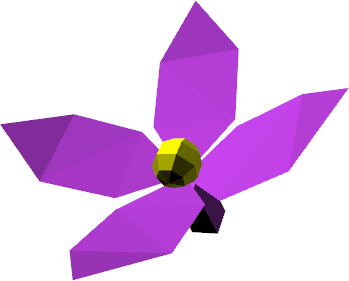
\includegraphics[scale=0.3]{Bloom4}}
	\subfloat[5th iteration]{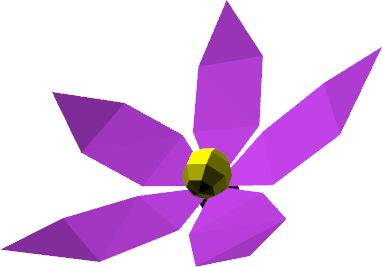
\includegraphics[scale=0.3]{Bloom5}}
	\subfloat[6th iteration]{
\includegraphics[scale=0.3]{Bloom6}}
	\\
	\subfloat[11th iteration of the Pythagoras tree]{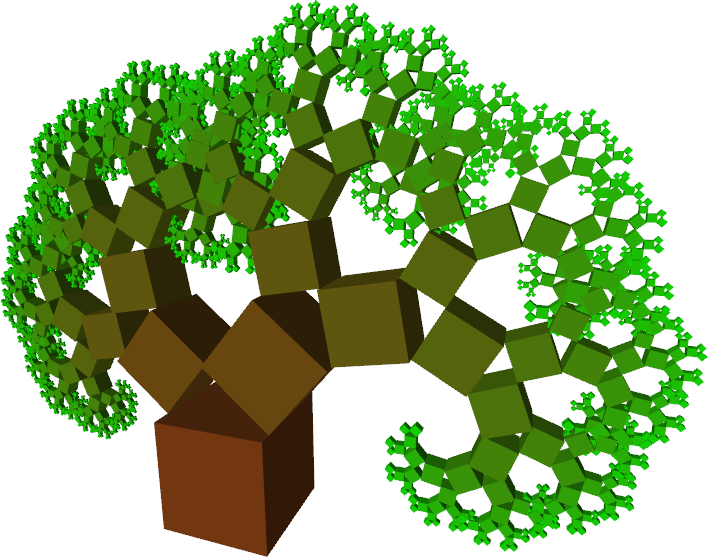
\includegraphics[width=0.55\textwidth]{Pythagoras}} ~
	\subfloat[3rd iteration of the Menger sponge]{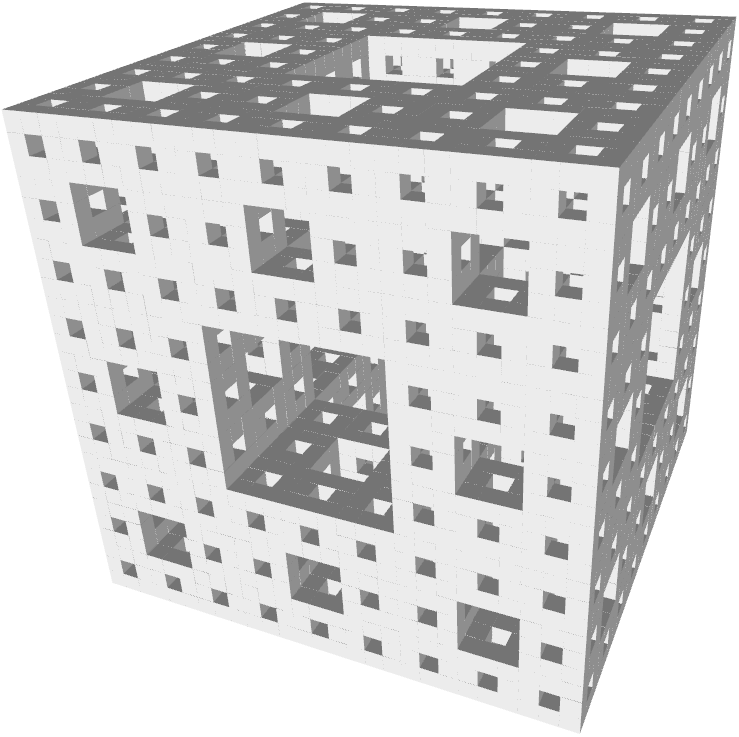
\includegraphics[width=0.40\textwidth]{MengerSponge}}
	\\
	\subfloat[The Pythagoras tree made of the Menger sponges with blossoms at the smallest cubes]{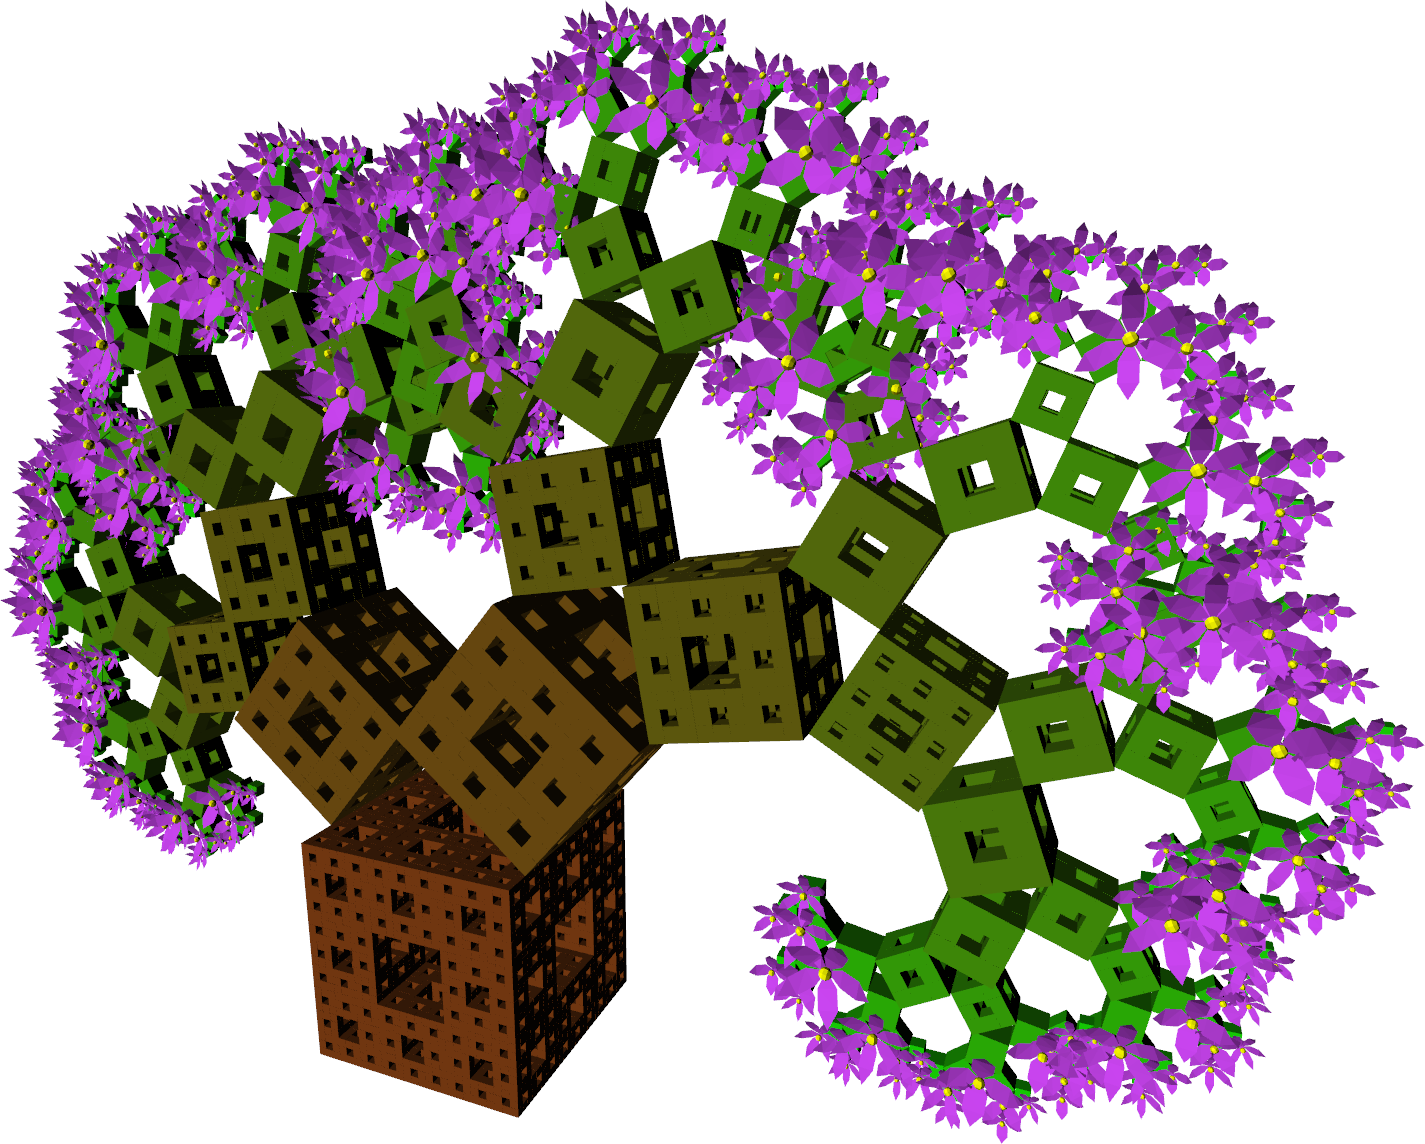
\includegraphics[width=0.9\textwidth]{HybridPythagoras}\label{fig:innerLsystemResult}}
	\caption{Example of interpreting s symbol as another \lsystem}
	\label{fig:innerLsystem}
\end{figure}

\begin{Lsystem}[label=lsys:innerLsystem,caption={Source code of \lsystem (Fig. \ref{fig:innerLsystemResult}) demonstrating use of an interpreting symbol as another \lsystem}]
lsystem HybridPythagorasTree(angle = 50) extends Branches {
	let angleComp = 90 - angle;  // angle complement
	let sinAngle = sin(deg2rad(angle));
	let sinAngleComp = sin(deg2rad(angleComp));
	set iterations = 8;
	set symbols axiom = F(64, 0);
	// interpret E(x) as DrawForward(x, x);  // cube
	@interpret E(x) as lsystem MengerSponge(x);@  // Menger sponge
	interpret m as MoveForward;
	interpret + as Yaw(angle);
	interpret - as Yaw(-angleComp);
	rewrite F(x)
		with left = x * sinAngle, right = x * sinAngleComp
		to E(x) [ + m(left / 2) F(right) ] - m(right / 2) F(left);
}

lsystem MengerSponge(size = 1) extends StdLsystem3D {
	let iters = if(size > 50, 2, if(size > 10, 1, 0));
	let cubeSize = size * (1/3)^iters;
	let renderBlooms = iters == 0;
	// add iteration to render blooms
	let iters = iters + if(renderBlooms, 1, 0);
	set iterations = iters;
	set symbols axiom = F;
	interpret F as DrawForward(cubeSize, cubeSize, #EEEEEE);
	interpret f as MoveForward(cubeSize / 2);
	@interpret B as lsystem Bloom(cubeSize);@  // renderes bloom
	rewrite F where renderBlooms to F [ ^ f B ];
	rewrite F to - f f + & f f ^ F F F +f+f- F F +f+f- F F +f+f- F
		-f+f+f^f F F &f&f^ F F &f&f^ F ^ ^ f f f & + f F F &f&f^ F
		^ ^ f f f & + f F F &f&f^ F ^ ^ f f f & + f F f & f f ^ +
		+ f f - f f f f f;
	rewrite f to f f f;
}

lsystem Bloom(size = 1) extends Polygons {
	let color = #d649ff;
	let leafCount = floor(random(4, 7));
	let angle = 150 / leafCount;
	set iterations = leafCount;
	set symbols axiom = F [ G(size/8) K ] leaf;
	interpret F as DrawForward(size * 0.5, size * 0.2, color);
	interpret G as MoveForward(size * 0.5);
	interpret K as DrawSphere(size / 6, #FFFF00);
	interpret + as Yaw(angle);
	interpret - as Yaw(-angle);
	interpret / as Roll;
	interpret ^ as Pitch(-15);
	rewrite leaf to /(360 / leafCount) [ ^(90) <(color) .
		+ ^ G . - ^ G . - ^ G . + +(180) + G . - ^ G .  > ] leaf;
}

process HybridPythagorasTree with ThreeJsRenderer;
\end{Lsystem}



\subsection{Final component system}

The final component system uses all the described functionality.
The component graph is shown in \autoref{fig:finalSystem}.
Two main \emph{process configurations} defined in the standard library use this scheme, namely the \hyperref[configurationSvgRenderer]{\emph{SvgRenderer}} and the \hyperref[configurationThreeJsRenderer]{\emph{ThreeJsRenderer}}
	(see appendix \ref{sec:stdLibProcessConfigurations}).

\begin{figure}[h!]
	\centering
	\begin{tikzpicture}[->,auto, node distance=3cm,>=latex,shorten >=2pt]
		\node (it) [block] {Iterator};
		\node (in) [block, above of=it, node distance=20mm] {Axiom provider};
		\node (rand) [block, below left of=it, node distance=28.284mm] {Random generator provider};
		\node (rw) [block, left of=it] {Rewriter};
		\node (caller) [block, right of=it, node distance=35mm] {Interpreter caller};
		\node (inter) [block, above of=caller, node distance=20mm] {Interpreter};
		\node (rend) [block, right of=inter] {Renderer};
		\node (out) [coord, right of=rend] {};
		\node (inner) [block, below of=caller, node distance=20mm] {Inner L-system processor};
				
		\draw (rw) to[bend left=40] (it);
		\draw (it) to[bend left=40] (rw);
		\draw (in) -- (it);
		\draw (it) -- (caller);
		\draw (it) -- (rand);
		\draw (caller) -- (inner);
		\draw [dashed] (caller) -- (inter);
		\draw (inter) -- (rend);
		\draw (rend) -- node {output} (out);
	\end{tikzpicture}
	\caption{Final component system}
	\label{fig:finalSystem}
\end{figure}


























\section{Web user interface}

The user interface is very important part of whole project.
To basic forms of user interface was considered, desktop application and web site.
The web was chosen because of following reasons.

\begin{description*}
	\item[Accessibility]
		Web is accessible on wide range of operating systems where desktop application can not be ported easily.
		Besides usual desktop systems it is possible to browse it on mobile devices like smart phones or tablets.		
	\item[No installation]
		End-user do not install anything, the application does not depend on user's OS.
		The solution is not easy to setup because it has many dependencies to third-party libraries.
		Web application is installed by experienced administrator and everything is set up properly.
	\item[Community]
		Users can share and discuss their work on the same place where they create it.
		This helps to create community which is important to all projects.
	\item[Up to date]
		Web user interface is always up to date.
		All updates are instantly applied for all users.
		Errors can be logged and administrator can fix them as soon as possible.		
\end{description*}

\begin{wrapfigure}{r}{0.4\textwidth}
	\vspace{-20pt}
	\includegraphics[width=\linewidth]{Sunflower}
	\caption{Logo of the web}
	\label{fig:logo}
	\vspace{-20pt}
\end{wrapfigure}

Web user interface also serve as comprehensive example of \lsystem processing library and its usage and capabilities.
Sunflower model in \autoref{fig:logo} was produced by the web site and because of its shape which fits in rectangle and good recognizability even as $32 \times 32$ pixels image it was chosen as the logo of the web page.

Web page have four main parts. First three parts, namely \emph{\lsystem processor}, \emph{Gallery of \lsystems} and \emph{Help} are accessible to anyone.
Fourth part is the \emph{Administration} and it is accessible only to administrators.

\subsection{\lsystem processor}

Main functionality of the web is processing of user's input (source code) and showing results.
For this purpose there is web page with big text area where the source code can be written.
There is three possibilities how to submit the source code.

First is processing source code and showing all results (or list of errors).
If there are too many outputs they are packed to one ZIP file.
All results can be downloaded.

Second possibility is to just compile source code and see compiled source code (no results are showed).
This is intended for debugging of errors in the input.

Last possibility which is available only for registered users is to save the source code.
To be able to save the source code successfully it must be without compilation errors.
For each saved source code unique is generated and it can be accessed by permanent link.
Saved inputs can be published in gallery.


\subsection{Gallery of \lsystems}

The gallery will serve as showcase of capabilities of \lsystems for new users as well as learning material.
All entries in gallery will have their source code included and anybody can try to process and customize it.
Registered users can rate other gallery entries.

Every registered user may contribute to gallery with their own creation.
To \lsystem into gallery user have to save and publish source code via \lsystem processor.
It is possible to alter thumbnail \lsystem over original \lsystem.
This allows to simplify images in thumbnail and show complex model in detail.

Tags can be assigned to each \lsystem in gallery.
Tag is short keyword, term or abbreviation which helps to describe \lsystem and allows it to be found again.
List of all tags can be listed and list of \lsystems filtered by specific tag can be shown.
Tag can contain short description of its meaning.
The description can be edited only by special user group.

\lsystems can be filtered also by user name.


\subsection{Help}

Important part of the web is the help.
Help contains few basic topics and FAQ (frequently asked questions) for new users.
Then there is list of predefined components, process configurations, constants, functions and operators.
Last part of the help is detailed syntax reference.


\subsection{Administration}

Administration section of the web is accessible to restricted group of users.
There is more administrators group every with different privileges.

The main administrators group is able to manage roles for all users, manage user groups (roles) and explore error logs.

Next group is able to explore all processed inputs on site, see all saved inputs and export input database to text file.

Last group can see list of submitted feedbacks and if the new feedback is submitted all users from this group will receive it via e-mail.


\subsection{Database}

The database will serve for saving all necessary data.
Figures \ref{fig:dbSchema1} and \ref{fig:dbSchema2} shows database scheme.
\emph{PK} after name means primary key and \emph{FK} foreign key.


\tikzstyle{db} = [draw, fill=blue!12, rectangle split, rectangle split parts=2]
\begin{figure}[p]
	\centering
	\begin{tikzpicture}[auto,>=latex]
		\node (user) [db, text width=6cm] {\textbf{User} \nodepart{second}
			UserId [Int32] (PK)\\
			Name [String] \\
			NameLowercase [String] \\
			PasswordHash [Binary] \\
			PasswordSalt [Binary] \\
			Email [String] \\
			RegistrationDate [DateTime] \\
			LastLoginDate [DateTime] \\
			LastActivityDate [DateTime] \\
			LastPwdChangeDate [DateTime]
		};
			
		\node (feedback) [db, below of=user, node distance=7cm, text width=6cm] {\textbf{Feedback} \nodepart{second}
			FeedbackId [Int32] (PK) \\
			UserId [String] (FK) \\
			Subject [String] \\
			SubmitDate [DateTime] \\
			Email [String] \\
			Message [String] \\
			IsNew [Bool]
		};
			
		\node (role) [db, above of=user, node distance=6cm, text width=6cm] {\textbf{Role} \nodepart{second}
			RoleId [Int32] (PK) \\
			Name [String] (FK) \\
			NameLowercase [String]
		};		
		
		\node (x) [coord, above right of=user, node distance=8cm] {};
		
		\node (vote) [db, above of=x, node distance=4cm, text width=6cm] {\textbf{Saved input vote} \nodepart{second}
			SavedInputId [Int32] (PK) \\
			UserId [Int32] (PK) \\
			Rating [Int32]
		};
		
		
		\draw [<-] (user) -- (feedback) node[pos=0.2]{0..1}  node[pos=0.55]{UserId}  node[pos=0.85]{*};
		\draw (role) -- (user) node[pos=0.2]{*}  node[pos=0.8]{*};
		\draw (vote) -- (x) node[pos=0.2]{*};
		\draw [->] (x) -- (user) node[pos=0.5]{UserId}  node[pos=0.8]{1};
		
		\draw [->] (x.east) -- +(3cm,0)  node[below,pos=0.5]{SavedInputId}  node[pos=0.8]{1}   node [xshift=1.5cm] {Saved inputs};
		\draw [<-] (user.east) ++(0,1cm) -- +(4cm,0) node[pos=0.2]{1}  node[below,pos=0.5]{CreationUserId}  node[pos=0.8]{*}   node [xshift=1.5cm] {Saved inputs};
		\draw [<-] (user.east) ++(0,-2cm) -- +(4cm,0) node[pos=0.2]{0..1}  node[below,pos=0.5]{UserId}  node[pos=0.8]{0..1}   node [xshift=1.5cm] {Input process};
		
	\end{tikzpicture}
	\caption{First half of the database scheme of the web}
	\label{fig:dbSchema1}
\end{figure}

\begin{figure}[p]
	\centering
	\begin{tikzpicture}[auto,>=latex]
		\node (input) [db, text width=6.5cm] {\textbf{Saved inputs} \nodepart{second}
			SavedInputId [Int32] (PK)\\
			UrlId [String] \\
			ParentInputProcessId [Int32] (FK) \\
			CreationUserId [Int32] (FK) \\
			CreationDate [DateTime] \\
			EditDate [DateTime] \\
			IsPublished [Bool] \\
			IsDeleted [Bool] \\
			PublishName [String] \\
			Views [Int32] \\
			SourceSize [Int32] \\
			OutputSize [Int64] \\
			Duration [Int64] \\
			MimeType [String] \\
			SourceCode [String] \\
			ThumbnailSourceExtension [String] \\
			Description [String] \\
			OutputMetadata [Binary] \\
			OutputThnMetadata [Binary] \\
			RatingSum [Int32] \\
			RatingCount [Int32]
		};
			
		\node (tag) [db, left of=input, node distance=7.5cm, text width=4.5cm] {\textbf{Tag} \nodepart{second}
			TagId [Int32] (PK) \\
			Name [String] \\
			NameLowercase [String] \\
			Description [String]
		};
			
		\node (proc) [db, below of=input, node distance=10cm, text width=6.3cm] {\textbf{Input process} \nodepart{second}
			InputProcessId [Int32] (PK) \\
			ParentInputProcessId [Int32] (FK) \\
			ChainLength [Int32] \\
			CanonicInputId [Int32] (FK) \\
			UserId [Int32] (FK) \\
			ProcessDate [DateTime] \\
			Duration [Int64]
		};
		
		\node (output) [db, below of=proc, node distance=6cm, text width=6cm] {\textbf{Process output} \nodepart{second}
			ProcessOutputId [Int32] (PK) \\
			InputProcessId [Int32] (FK) \\
			FileName [String] \\
			CreationDate [DateTime] \\
			LastOpenDate [DateTime] \\
			Metadata [Binary]
		};
		
		\node (canonic) [db, xshift=-1cm,  below left of=proc, node distance=8.5cm, text width=5.3cm] {\textbf{Canonic input} \nodepart{second}
			CanonicInputId [Int32] (PK) \\
			Hash [Int32] \\
			SourceCode [String] \\
			SourceSize [DateTime] \\
			OutputSize [DateTime]
		};
		
		
		\draw (input) -- (tag)  node[pos=0.2]{*}  node[pos=0.8]{*};
		\draw [->] (input) -- (proc)  node[pos=0.2]{*}  node[pos=0.5]{ParentInputProcessId}  node[pos=0.8]{0..1};
		\draw [<-] (proc) -- (output)  node[pos=0.2]{0..1}  node[pos=0.6]{InputProcessId}   node[pos=0.9]{*};
		\draw [->] (proc) -- (canonic)  node[pos=0.08]{*}  node[pos=0.35]{CanonicInputId}   node[pos=0.65]{1};
		\draw [->] (proc) edge [in=180,out=190,loop] node[pos=0.15]{0..1}  node[pos=0.5]{ParentInputProcessId}   node[pos=0.9]{*} ();
		
		\draw [<-] (input.west) ++(0,4cm) -- +(-4cm,0) node[above,pos=0.2]{1}  node[below,pos=0.5]{SavedInputId}  node[above,pos=0.8]{*}   node [xshift=-2cm] {Saved input vote};
		\draw [->] (input.west) ++(0,-4cm) -- +(-4cm,0) node[above,pos=0.2]{1}  node[below,pos=0.5]{CreationUserId}  node[above,pos=0.8]{*}   node [xshift=-1cm] {User};
		\draw [->] (proc.west) ++(0,1cm) -- +(-4cm,0) node[above,pos=0.2]{0..1}  node[below,pos=0.5]{UserId}  node[above,pos=0.8]{0..1}   node [xshift=-1cm] {User};
	\end{tikzpicture}
	\caption{Second half of the database scheme of the web}
	\label{fig:dbSchema2}
\end{figure}


In the left part of the scheme (\autoref{fig:dbSchema1}) are tables \emph{User} and \emph{Roles} with relation \emph{n} to \emph{n} (any user can be in any number of roles).
both tables table contains column called \emph{NameLowercase} for canonical representation of user names for easier searching.
\emph{Feedback} table for saving posted feedback have foreign key to \emph{Users} (if registered user submit a feedback).

The right part of the scheme is (\autoref{fig:dbSchema2}) more complicated.
Every processed input is saved to the \emph{Input process} table.
To optimize size of the database the source code is not saved for every input process but it is canonicalized and saved to the \emph{Canonic input} table.
Hash is counted for every saved canonical input to speed up lookup for identical inputs.
This system ensures that in the database will not be saved two identical source codes.
One might thing that the probability of processing two identical source codes is very low but it is not true.
The most users trying to process \lsystems from gallery and do minor changes to them like changing number of iterations.

Results of processing (like images) are not saved directly to database because they are relatively big.
They are saved to local disk to working directory (which can be configured).
To ensure correct cleaning of files in the working directory there is table called \emph{Process output}.
Record of each produced file is saved into this table.
If file is viewed by user the \emph{LastOpenDate} entry is updated.
If the number of stored files exceeds maximum (which can be configured) the files with the longest time before last opening are deleted.
This mechanism allows to keep alive old but viewed files with no need to saving them permanently (for example for sharing with friend).

Moreover the new files are saved with the \emph{LastOpenDate} lowered by one minute over the \emph{CreationDate}.
This will cause that deleting of non-viewed files is likely than viewed ones.
It can protect wiping all input from database by some bot who do not open processed outputs.

Lets get back to saving of all processed inputs to the \emph{Input process} table.
If user is creating \lsystem the process is iterative.
Parent input processes are saved (in \emph{ParentInputProcessId}) as user develops the \lsystem.
This set of processes forms a chain.
The longer the chain of processes is the better can be expected.
The length of a chain can be counted by searching the database an resolving the \emph{ParentInputProcessId} column.
However this process can take very long time because the \emph{Input process} table will likely have many rows.
To be possible to easily find longest chains the chain length is counting for each row in column \emph{ChainLength}.

If new input is about to save to the \emph{Input process} table and it do not have parent (for example first process after opening the page) the \emph{Canonic input} table is searched for corresponding input.
If the canonical input it is found the oldest\footnote{More input process entries can share one canonical input entry.} corresponding input process is selected as the parent.


\subsubsection{Saved inputs}

Registered users can save their inputs.
They are saved to the \emph{Saved inputs} table which also serves as table for the gallery.
For every saved input is generated unique ID stored in the \emph{UrlId} column.
This is is used in the permanent link which allows permanent access to all saved inputs.

Saved inputs can be edited by owner but more importantly the can be published to the gallery.
In the gallery inputs can be rated.
For this is table \emph{Saved input vote}.
Primary key to this table is pair of \emph{SavedInputId} and \emph{UserId} allowing each user to vote to every input just once (of course the vote can be changed).

Published entries in the \emph{Saved inputs} table are sorted by average rating taking into account total number of votes (the more votes the better).
To speed the sorting and eliminate joining with the \emph{Saved input vote} table the sum and the count of votes is stored directly in the \emph{Saved inputs} table.

Source code of saved inputs is saved as is (without any canonicalization) to preserve comments and formatting.
To allow generating thumbnail different from the original image and to save space and user effort the thumbnail is generated by adding content of the \emph{ThumbnailSourceExtension} to the \emph{SourceCode}.
Because the last result is saved the source code in the \emph{ThumbnailSourceExtension} can produce thumbnail easily with usage of next process statement.























































